\documentclass[spanish]{article}
\usepackage[spanish]{babel}
\usepackage{amsmath}
\usepackage{amssymb}
\usepackage[utf8]{inputenc}
\usepackage{vmargin}
\usepackage{graphicx}
\usepackage{wrapfig}
\usepackage[export]{adjustbox}


\begin{document}
	\setpapersize{USletter}
	\setmarginsrb{30mm}{30mm}{30mm}{30mm}{0pt}{0mm}{0pt}{0mm}
	\begin{center}
	{\Large Análisis de Algoritmos, Sem: 2018-1, 3CV2 Práctica 4, 14 de Septiembre del 2017}\\
	{\huge {\bf Práctica 4: Divide y Venceras: Algoritmo QuickSort.}} \\
	{\large {\bf Luis Daniel Martinez Berumen}}\\
	
\includegraphics[width=1\textwidth]{./imagenes/logos.png}\\

\end{center}

	\bigskip
	
	\bigskip
	
	\bigskip
	
	{\LARGE {\bf Abstract}}\\
En esta practica vamos a demostrar, tanto de manera analitica como de manera practica con graficas de los experimentos, como los algoritmos Partition y el QuickSort tienen complejidad complejidad lineal, para el Partition y el QuickSort con complejidad  $\theta$ (nlogn), todo esto con ayuda del paradigma de Divide y Venceras el cual nos ayudara a el analisis de cada uno de los algoritmos, ademas de mostrar la resolucion de 2 problemas en la parte de anexos.
\bigskip

	{\Large {\bf Palabras Clave}}\\
	\begin{itemize}
		\item Algoritmo
		\item Funcion
		\item Orden
		\item Recursividad
		\item Paradigma
	\end{itemize}
	
	\section{Introducci\'on}
	Divide y Vencerás es una frase quye hemos escuchado todos, al menos, una vez en nuestra vida, para nosotros 
	es técnica de diseño de algoritmos, siendo de gran utilidad para nuestra carrera, ya que, 
	los problemas a los que nos enfrentamos día con día son mas faciles de resolver si aplciamos una tecnica de este tipo.
	De hecho, suele ser considerada una filosofía general para resolver problemas, no solo del termino informatico, sino que también se utiliza en muchos otros ámbitos

\newpage

	\section{Conceptos B\'asicos}
	Para la correcta comprension de este trabajo, es necesario definir algunos terminos tales como $\theta$, O y $\Omega$.\\
	 $\theta$(n):\\
		Sea g(n) una función. Se define  $\theta$ (g(n)) como:\\
		
		 	$\theta$(g(n)) = $\{ f(n) \quad | \quad \exists c1,c2>0 \quad \& \quad n_{0}>0 \quad \mid \quad \forall n>=n_{0} \quad 0<= c1g(n) <= f(n) <= c2g(n) \}$
	\bigskip		 	
		 	
	O(n):\\
		Sea  g(n)  una función, O(n) (el pero de los casos) se define como:\\
		
			\hspace{1cm}O(n)=$\{f(n) \quad | \quad \exists c >0 \quad \& \quad n_{0}>0 \quad | \quad f(n) <= Cg(n) \quad \forall  n>= n_{0} \}$
	\bigskip
	
	$\Omega$(n):\\
	Sea  g(n)  una función. Se define $\Omega$ (g(n)) (el mejor de los casos) como:\\

		\hspace{1cm}$\Omega$(g(n)) =$\{f(n) \quad | \quad \exists c >0 \quad \& \quad n_{0}>0 \quad \mid \quad  0<= cg(n)<= f(n) \quad \forall n>= n_{0} \}$
	\bigskip

	El ordenamiento rápido (quicksort en inglés) es un algoritmo basado en la técnica de divide y vencerás, que permite, en promedio, ordenar n elementos en un tiempo proporcional a n log  		. Esta es la técnica de ordenamiento más rápida conocida. Fue desarrollada por C. Antony R. Hoare en 1960. El algoritmo original es recursivo, pero se utilizan versiones iterativas para 		mejorar su rendimiento (los algoritmos recursivos son en general más lentos que los iterativos, y consumen más recursos).
	El algoritmo fundamental es el siguiente:

	\begin{itemize}
		\item Elegir un elemento de la lista de elementos a ordenar, al que llamaremos pivote.
		\item Resituar los demás elementos de la lista a cada lado del pivote, de manera que a un lado queden todos los menores que él, y al otro los mayores. En este momento, el pivote 				ocupa exactamente el lugar que le corresponderá en la lista ordenada.
		\item La lista queda separada en dos sublistas, una formada por los elementos a la izquierda del pivote, y otra por los elementos a su derecha.
		\item Repetir este proceso de forma recursiva para cada sublista mientras éstas contengan más de un elemento. Una vez terminado este proceso todos los elementos estarán 				ordenados. Como se puede suponer, la eficiencia del algoritmo depende de la posición en la que termine el pivote elegido.
		\item En el mejor caso, el pivote termina en el centro de la lista, dividiéndola en dos sublistas de igual tamaño. En este caso, el orden de complejidad del algoritmo es O(n·log n).
		\item En el peor caso, el pivote termina en un extremo de la lista. El orden de complejidad del algoritmo es entonces de $0(n^{2})$. El peor caso dependerá de la implementación del algoritmo, aunque habitualmente ocurre en listas que se encuentran ordenadas, o casi ordenadas.
		\item En el caso promedio, el orden es O(n·log n).
	\end{itemize}

	\bigskip
	\begin{center}
		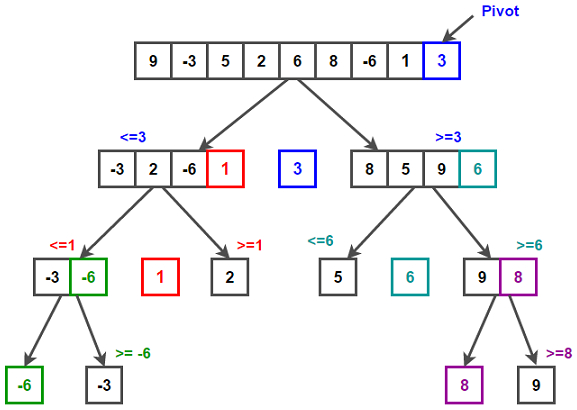
\includegraphics[width=100mm]{./imagenes/Quicksort.png}\\
		Figura 1: QuickSort
	\end{center}

	\newpage	

	\bigskip
\section{Experimentaci\'on y Resultados}
	
	\subsection{Implemente el algortimo QuickSort}
	
	{\large i)Mediante graficas, muestre que el algoritmo {\bf Partition} tiene complejidad lineal.}\\
	
	\bigskip

	Para empezar este ejercicio tomamos arreglos creciendo iterativamente de tamaño 1 hasta el 50, llenandolos con valores 			aleatorios no repetidos segun su tamaño.
	Para esta prueba, el algoritmo Partition arrojo los siguientes resultados

	\begin{center}
	\includegraphics[scale=.5]{./imagenes/tpar/1.png}\\
	\includegraphics[scale=.5]{./imagenes/tpar/2.png}\\
		Figura 2: Tabla de Partition.
	\end{center}
\newpage
	Para estos resultados, se realizo una grafica confrontando los resultados tabulados anteriormente, la cual quedo de la siguiente manera.\\
	\begin{center}
		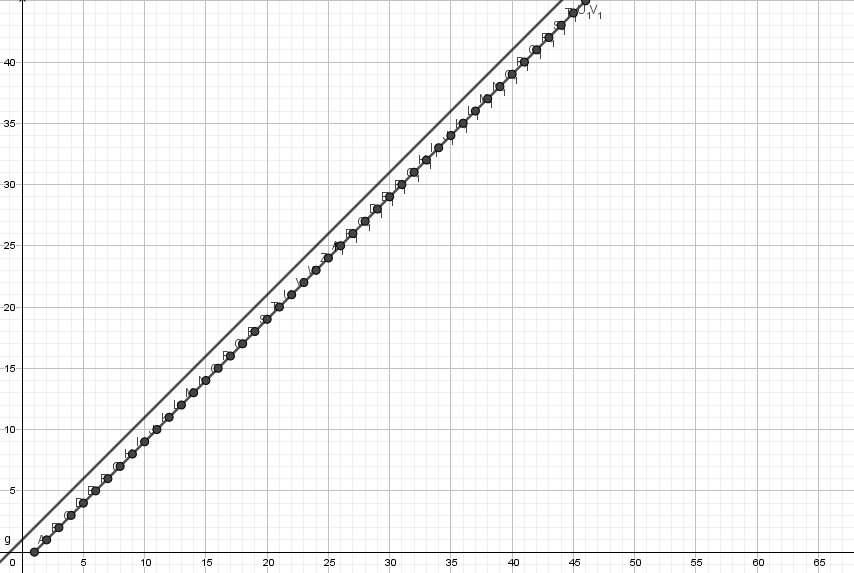
\includegraphics[scale=.5]{./imagenes/partition.png}\\
		Figura 3: Grafica de Partition.
	\end{center}
	Podemos concluir que nuestra funcion es lineal ya que al compararala con una funcion que se multiplica con una constante es evidente el caracter de la funcion no solo por los resultados obtenidos en la tabla de paso, si no, tambien por la grafica que generamos.
	\bigskip
\newpage
	{\large ii)Demostrar analiticamente que el algortimo {\bf Partition} tiene complejidad lineal.}\\
	
	\bigskip
		Sea n = r-q-1;
	\bigskip
	
	Partition \\
	Entrada: A[p,...,r],p,r;\\
	Salida : q
	\bigskip
	
	Partition(A,p,r)\\
	$
	\left.
	\begin{array}{l}
		\hspace{0.2cm}1.-x=A[r-1]\\
		\hspace{0.2cm}2.-i=\quad p-1\\
	\end{array}
	\right\rbrace
	\theta(1);
	\\
	{\setlength{\parindent}{-5cm}
	\left.
	\begin{array}{l}
		\left.
		\begin{array}{l}
			3.- for \quad j=p \quad  to \quad  j<= r-2 \quad do \\
		\end{array}
		\right\rbrace
		\theta(n);
		\\
		\left.
		\begin{array}{l}
			4.- \hspace{0.7cm} if \quad A[j]<=x \\
			5.- \hspace{1.4cm} i=i+1 \\
			6.- \hspace{1.4cm} intercambio(A[j],A[i]) \\
		\end{array}
		\right\rbrace
		\theta(1);
		\\
	\end{array}
	\right\rbrace
	\theta(1*n)=O(n);
	}
	\\
	\left.
	\begin{array}{l}
		\hspace{0.2cm}7.- intercambio(A[i+1],A[r-1])\\
		\hspace{0.2cm}8.- return \quad i+1\\
	\end{array}
	\right\rbrace
	\theta(1);
	\bigskip
	\\	
	O(1)  +  O(n)+  O(1) =  O(1) +  O(n)=O(max\{1,n\})=O(n)$ \\
	Como podemos notar para el mejor de los casos el orden de complejidad tambien es lineal.\\
	$\therefore T(n) = \theta(n).$
	\bigskip	
	\newpage

	{\large  iii)Mostrar mediante graficas, que el algoritmo {\bf QuickSort} tiene complejidad $\theta(nlogn)$.}\\
	
	\bigskip
	Para empezar este ejercicio tomamos arreglos creciendo iterativamente de tamaño 1 hasta el 50, llenandolos con valores 			aleatorios no repetidos segun su tamaño.
	Para esta prueba, el algoritmo QuickSort arrojo los siguientes resultados
	\begin{center}
	\includegraphics[scale=.5]{./imagenes/tqs/1.png}\\
	\includegraphics[scale=.5]{./imagenes/tqs/2.png}\\
		Figura 4: Tabla de QuickSort.
	\end{center}
\newpage
	Para estos resultados, se realizo una grafica confrontando los resultados tabulados anteriormente, la cual quedo de la siguiente manera.\\
	\begin{center}
		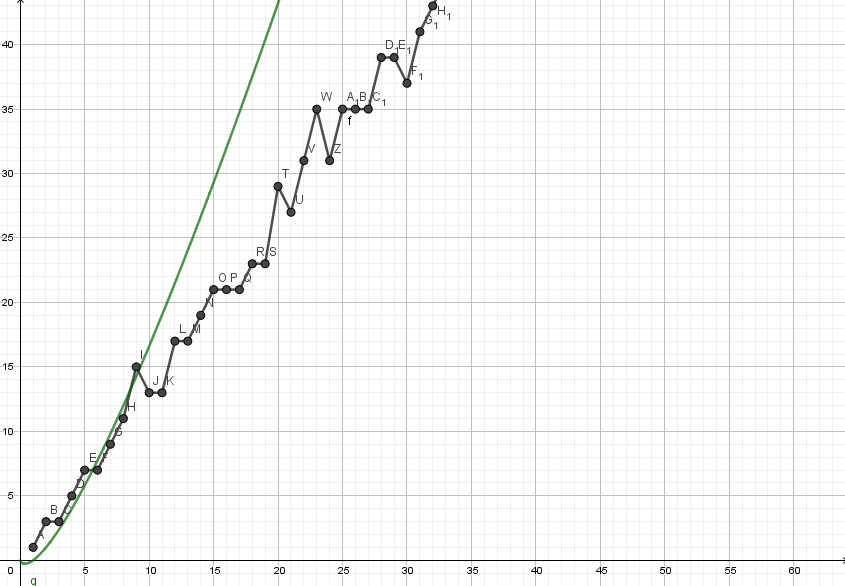
\includegraphics[scale=.5]{./imagenes/qs.png}\\
		Figura 5: Grafica de QuickSort.
	\end{center}
	
	La figura numero 5 es la conclucoin a todas nuestras pruebas y a nuestros desarrollos podemos observar que el inicio de las curvas es el mismo mientras que cuando los valores de nuestro quicksort empiezan a desvariar, creemos que esta variacion es debido a los valores obtenidos por el random para llenar los arreglos, muchas veces se generan complejidades menores , como seria el caso de 1,2,3,4,5,6,..., n donde el arreglo se encuentra, si no en su totalidad ordenado, si en una parte, lo cual, creo que podria interferir con los resultados, sin embargo, se deduce que la complejidad del algoritmo QuickSort es de $\theta$(nlogn), debido a las graficas obtenidas y su similitud.

	\bigskip
\newpage
	{\large  iv)Demostrar analiticamente que el algoritmo {\bf QuickSort} tiene complejidad  $\theta(nlogn)$ cuando el pivote divide el arreglo por la mitad. }\\		

	\bigskip
	Sea n = r-p;
	\bigskip
	
	QUICKSORT\\
	Entrada: A[p,...,r],p,r;\\
	Salida : A[p,...,r] ordenado
	
	QuickSort(A,p,r)\\
	1.- if(p!=r)\\
	2.-\hspace{0.7cm}$q \leftarrow Partition(A,p,r)$;\\
	3.-\hspace{0.7cm}QuickSort(A,p,q);\\
	4.-\hspace{0.7cm}QuickSort(A,q+1,r);\\
	\bigskip
	
	Sea G(n) la complejidad del algoritmo de Partition demostrado anteriormente, es decir $\theta(n)$.\\
	Entonces sea T(n) la complejidad del algoritmo de Quicksort la cual se define como:\\
	T(n) = G(n) + T(q) + T(n-q) cuando $n>1$.\\
	Como el pivote divide el arreglo a la mitad entonces q=n/2.\\
	\\
	Con ello\\
	T(n) = 
	$
		\left\lbrace
		\begin{array}{l}
			\theta(1) \quad si \quad n = 1;\\
			2T(n/2) + G(n) \quad si \quad n>1 \quad con \quad n = 2^{k}\\
		\end{array}
		\right.
	$	
	\bigskip
	
	Es decir\\
	T(n)
	$
		\left\lbrace
		\begin{array}{l}
			c \quad si \quad n = 1;\\
			2T(n/2) + c*n \quad si \quad n>1 \quad  con  \quad n = 2^{k}\\
		\end{array}
		\right.
	$
	\bigskip
	
	Como $n = 2^{k}$ entonces:\\
	$T(2^{k})=2T(2^{k-1}) + c(2^{k})$\\
	$T(2^{k})=2[2T(2^{k-2}) + c(2^{k-1})] + c(2^{k})$\\
	$T(2^{k})=4T(2^{k-2}) + 2c(2^{k})$\\
	$T(2^{k})=4[2T(2^{k-3}) + c(2^{k-2})]+ 2c(2^{k})$\\
	$T(2^{k})=8T(2^{k-3}) + 3c(2^{k})$\\
	\hspace{1cm}\vdots\\
	$T(2^{k})=(2^{i})T(2^{k-i}) + ic(2^{k})$\\
	Cuando i = k\\
	$T(2^{k})=(2^{k})T(2^{k-k}) + kc(2^{k})$\\
	$T(2^{k})=(2^{k})c + kc(2^{k})$\\
	Remplazando $2^{k} = n \quad y \quad k=\log_{2}(n)$\\
	$T(n)=cn + c(n\log_{2}(n))$\\
	$T(n)=c(n + n\log_{2}(n))$\\
	$\therefore \quad T(n) = \theta(n\log_{2}(n))$	
	
	\bigskip
\newpage
	{\large  v)Mediante graficas, proponga el orden de complejidad de QuickSort cuando todos los elementos del arreglo son distintos y estan ordenados en forma decreciente. }\\
\bigskip
	Para empezar este ejercicio tomamos arreglos creciendo iterativamente de tamaño 1 hasta el 50, llenandolos con valores 			decrecientes con el mayor igual al tamaño del arreglo.
	Para esta prueba, el algoritmo QuickSort arrojo los siguientes resultados
 \begin{center}
	\includegraphics[scale=.5]{./imagenes/tqsDesc/1.png}\\
	\includegraphics[scale=.5]{./imagenes/tqsDesc/2.png}\\
		Figura 6: Tabla de QuickSort con orden decreciente.
	\end{center}
\newpage
	Para estos resultados, se realizo una grafica confrontando los resultados tabulados anteriormente, la cual quedo de la siguiente manera.\\
	\begin{center}
		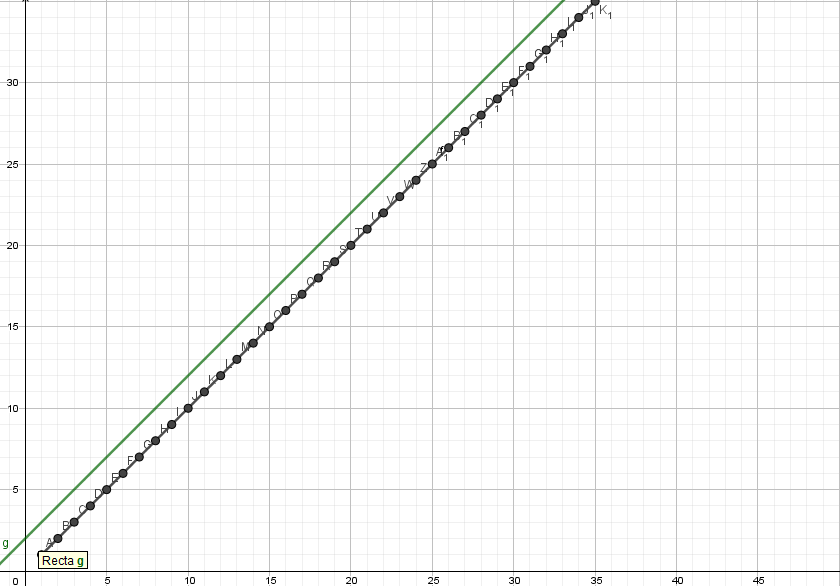
\includegraphics[scale=.5]{./imagenes/qsDec.png}\\
		Figura 7: Grafica de QuickSort con orden decreciente.
	\end{center}
	Para estos resultados llegue a la conclusion de que el orden es lineal, ya que es un caso especial del quicksort, por la forma en la que estan acomodados los valores, esmas sencillo para el algoritmo lograr acomodarlos, lo que nos deja con una complejidad de tipo lineal, debido a los datos obtenidos con la comparacion de graficas, se llega a la conclucion de que el algoritmo QuickSort con datos decrecientes es de complejidad lineal.
		
	\bigskip

	\newpage

	\bigskip

	\section{Conclusi\'on}

	\bigskip
En esta pracitca observe que dependiendo de el tipo de datos que se introduzcan a un algoritmo de ordenacion como QuickSort, dependera el tiempo computacional que tarde en ordenarlo, debido a su funcionamiento.\\Comenzamos a ver algoritmos mas y mas complejops, que, ademas de su complejidad debido a la recusividad, son ahora dependientes de los valores con los que se va a  probar.\\Tuve algunos problemas debido al las graficas de quicksort, intentaba tabular 200 resultados, pero los valores cambiaban demasiado, no lograba entender que sucedia hasta que decidi imprimir cada arreglo antes y despues de ordenarlo, imprimiendo igual las veces que se ejecuto el algoritmo QuickSort, fue entonces cuando note que lops algoritmos que tenian valores ya ordenados, aunque fuera en una parte solamente, tardaban menos pasos en ser ordenados en su totalidad, por lo tanto, reduje el tamaño de las pruebas para lograr reducir este fallo.

	\bigskip

	\newpage

	\section{Anexos:}
	
	\subsection{Resolver los siguientes problemas:}

	{\large 1. Que valor de q retorna {\bf Partition} cuando los elementos del arreglo $A[p, ... ,r]$ tienen el mismo valor?}\\\\
	Con este experimento, donde pusimos los arreglos llenos de 1, pudimos ver que el valor que Partition nos regresa es igual al tamaño del arreglo mismo. Esto lo podemos garantizar por lo que vemos en la figura 8, los arreglos en este experimento fueron tomados del 1 al 50.\\\\\\\\
	{\large 2.Cual es el tiempo de ejecucion de {\bf QuickSort} cuando todos los elementos del arreglo tienen el mismo valor?}\\\\
	Del mismo modo, la tabulacion obtenida suguiere que la complejidad obtenida por el algoritmo QuickSort con datos iguales, es de complejidad lineal.
 \begin{center}
	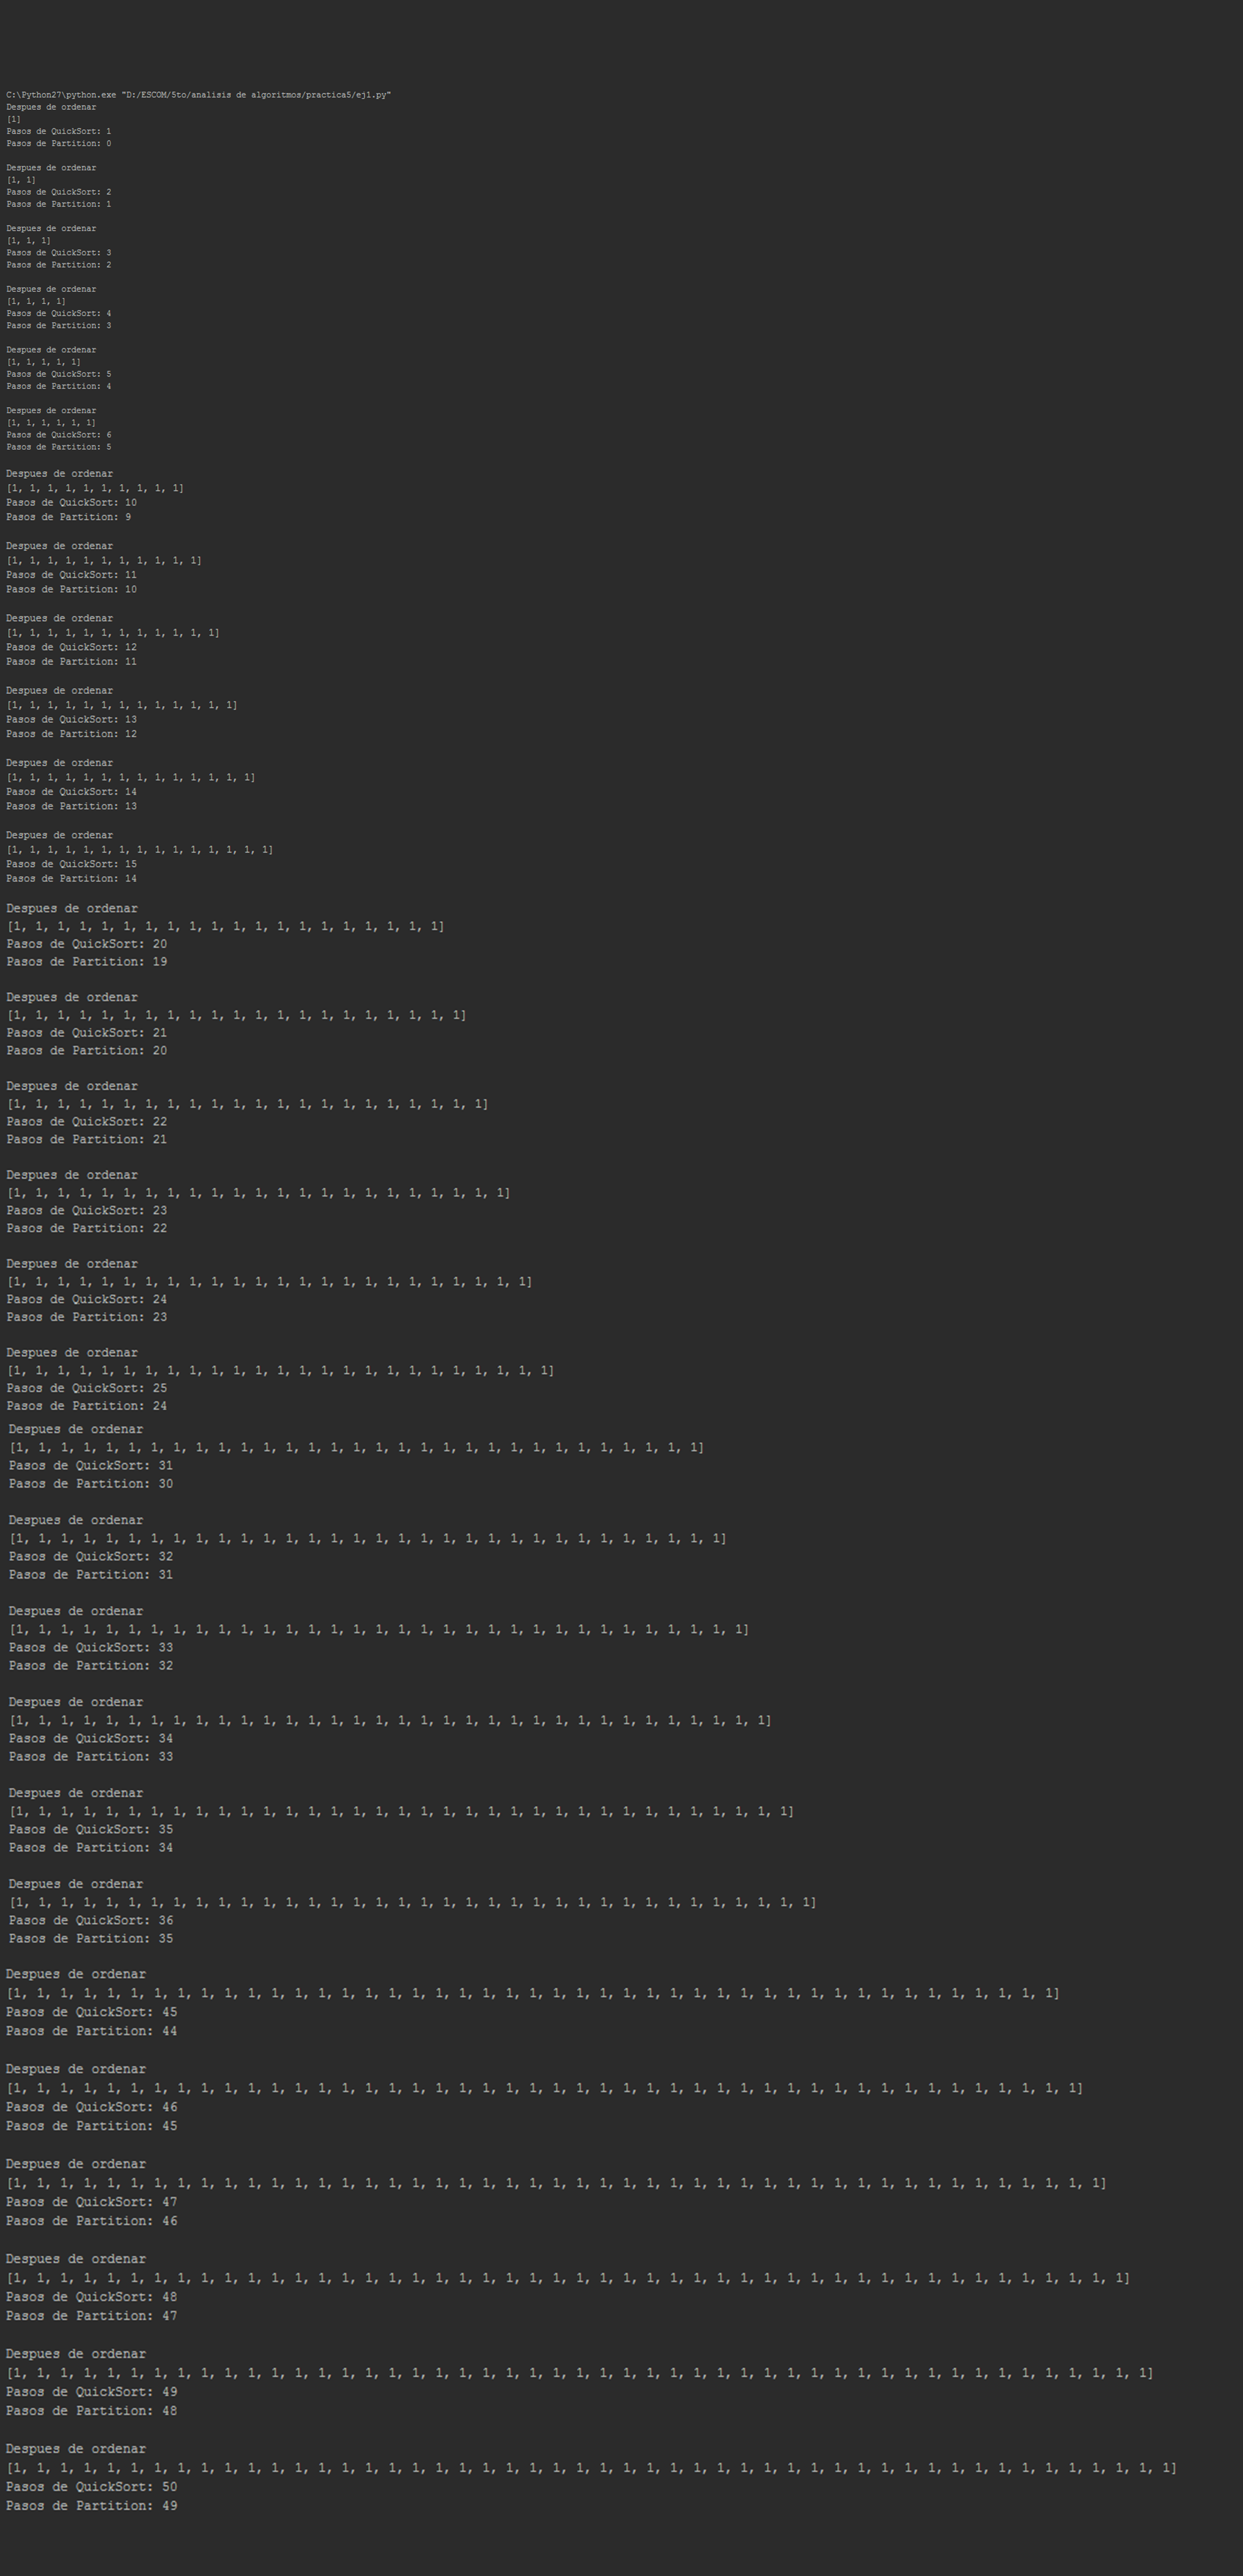
\includegraphics[scale=.5]{./imagenes/anexos.png}\\
		Figura 8: Tabla de QuickSort con orden numeros iguales.
	\end{center}

	\bigskip
\end{document}